\chapter{SR Sensível ao Tempo}\label{chapter:proposta}

Neste capítulo é apresentado o SR Sensível ao Tempo para ambientes educacionais proposto nesse trabalho. O algoritmo proposto
considera o decaimento nos interesses do usuário com o passar do tempo (categoria do Decaimento - Seção \ref{section:decay}). Além
do algoritmo proposto, são apresentados cenários que ilustram o uso desse algoritmo e discussões sobre as suas vantagens.

\section{Algoritmo Proposto}\label{section:algoritmo-proposto}

O algoritmo de recomendação proposto nesse trabalho combina a Abordagem Baseada em Conteúdo com o uso do
contexto temporal através da categoria Decaimento (ver seção \ref{section:decay}). Para o SR, o perfil do usuário é composto pelos
itens acessados por ele. A cada item acessado pelo usuário, são armazenadas as palavra-chaves
do item juntamente com a posição desse item no histórico do usuário, começando em $1$ para o
primeiro item acessado. Os itens que serão recomendados também são representados no algoritmo de recomendação por um conjunto de palavras-chave. O cálculo da
relevância de um determinado item $i$ para um usuário $u$ no algoritmo proposto está representado na Equação \ref{eq:relevancia-proposta}.

\begin{equation}
  F(u,i) = S(u,i) \cdot R(I_{u,i}) + A(i)
  \label{eq:relevancia-proposta}
\end{equation}

Onde: $F$ é a função que calcula a relevância de um item $i$ para um usuário $u$; $S$ é a função de similaridade entre
o perfil do usuário $u$ (representado através de conjunto de palavras-chave dos itens acessados) e o item $i$
(representado pelo conjunto de palavras-chave que o caracterizam); $R$ é o maior valor de recência dos itens do conjunto
$I_{u,i}$ (itens acessados pelo usuário $u$ e com alguma similaridade com o item $i$); $A$ é uma função que retorna $1$
se o item $i$ nunca foi acessado pelo usuário $u$ e $0$ se o item já foi acessado.  O valor da relevância
varia entre zero (menor relevância) e dois (maior relevância), e os itens com maior valor de $F$ serão recomendados.

A função $S$ de similaridade entre o usuário $u$ e o item $i$ pode ser calculada utilizando funções de similaridade como
o Cosseno (ver Seção \ref{subsection:baseada-em-conteudo}). A função de recência $R$, responsável pelo Decaimento, está definida na Equação
\ref{eq:recencia-proposta}.

\begin{equation}
  R(I_{u,i}) = \max_{\{j \in I_{u,i}\}}{\frac{x_j}{\left| I_u \right|}}
  \label{eq:recencia-proposta}
\end{equation}

Onde: $x_j$ é a posição do item $j$ na lista de itens acessados pelo usuário $u$ ordenada pela ordem de acesso;
e $\left| I_u \right|$ é a quantidade de itens acessados pelo usuário $u$. Essa fórmula considera
que mais de um item acessado pelo usuário pode ser similar ao item $i$, por isso a fórmula retorna a maior recência de
todos os itens presentes no perfil do usuário que são similares a $i$. A seguir temos um exemplo do uso da fórmula da
recência considerando apenas um item, que pode ser estendida para o uso com vários itens e aplicada a função $max$ como descrito na
fórmula acima.

Considerando um usuário $u$ que acessou três itens A, B e C com as seguintes posições: Item A - posição 2, Item B - posição 1 e
Item C - posição 3. Supondo que o item candidato $i$ a ser recomendado seja similar aos itens B e C, a Recência desse item, calculada
utilizando a equação apresentada anteriormente, seria $1.0$ como pode ser vista na Equação \ref{eq:recencia-item-candidato}.

\begin{equation}
  R(i) = \max{(\frac{1}{3}, \frac{3}{3})} = 1.0
  \label{eq:recencia-item-candidato}
\end{equation}

No Algoritmo \ref{alg:proposta-pseudocodigo} é possível observar o pseudocódigo do algoritmo proposto. Nesse algoritmo
estão representadas em mais alto nível as etapas da recomendação. Primeiramente, são buscados no banco de dados os itens acessados
pelo usuário e os itens candidatos à recomendação. Os itens candidatos à recomendação podem ser todos os itens disponíveis
no ambiente ou um subconjunto de itens, de acordo com a necessidade da aplicação.

O cálculo da recência para cada item do perfil do usuário é feito também na fase de inicialização, pois esse cálculo só
precisa ser realizado uma vez. Depois disso, para cada item candidato a ser recomendado para o usuário, é calculada a
similaridade do perfil do usuário (composto pelas palavras-chave dos itens acessados por ele) com as palavras-chave do item
candidato. Além disso, é buscada a lista de itens acessados pelo usuário que são similares ao item candidato. Nessa etapa, também é
encontrado o Item Acessado pelo usuário mais recente que é similar ao item candidato, para utilizar o seu valor de recência no cálculo da Relevância.
O cálculo da Relevância para o item candidato é realizado utilizando a Equação \ref{eq:relevancia-proposta}.

\begin{algorithm}
  \caption{Pseudocódigo do Algoritmo de Recomendação Proposto. \label{alg:proposta-pseudocodigo}}

  \SetKwInOut{Input}{input}
  \SetKwInOut{Output}{output}
  \SetKwProg{algoritmoRecomendacaoDecay}{algoritmoRecomendacaoDecay}{}{}

  \algoritmoRecomendacaoDecay{$(Usuário)$}{
    \Input{Usuário que irá receber a recomendação.}
    \Output{Lista com cinco itens recomendados para o usuário.}
    \tcc{Inicialização}
    itens = buscarItensCandidatos()\;
    itensAcessados = buscarItensAcessados(Usuário)\;
    recênciaItensAcessados = calcularRecência(itensAcessados)\;
    relevâncias = \{\}\;
    \tcc{Computação das recomendações}
    \ForEach{$item \in itens$}{
      similaridade = calcularSimilaridade(itensAcessados, item)\;
      itensSimilares = buscarItensSimilares(itensAcessados, item)\;
      recência = calcularMaxRecência(itensSimilares, recênciaItensAcessados)\;
      relevâncias[item] = similaridade * recência + itensAcessados.inclui?(item)\;
    }

    \Return relevâncias.max(5)\;
  }
\end{algorithm}

No Algoritmo \ref{alg:calcular-recencia-pseudocodigo} é demonstrado o cálculo da recência para cada um dos itens do perfil do
usuário, que é utilizado pelo Algoritmo \ref{alg:proposta-pseudocodigo} descrito anteriormente. Para esse cálculo, o próprio registro
de item acessado pelo usuário possui a informação da posição em que se encontra no histórico do usuário e é aplicada
uma versão simplificada da Equação \ref{eq:recencia-proposta}. A função $max$ presente na Equação \ref{eq:recencia-proposta}
não é aplicada nesse momento, sendo calculada apenas a recência
para cada item individualmente. No método descrito no Algoritmo \ref{alg:max-recencia-pseudocodigo} é que a função $max$ será
aplicada para encontrar a maior recência entre os itens similares ao item candidato à recomendação. O algoritmo tem um processo
que difere da Equação \ref{eq:recencia-proposta} justamente para que recência não seja recalculada várias vezes e assim
melhore o seu tempo de processamento.

\begin{algorithm}
  \caption{Pseudocódigo do cálculo da recência para cada item presente no perfil do usuário. \label{alg:calcular-recencia-pseudocodigo}}

  \SetKwInOut{Input}{input}
  \SetKwInOut{Output}{output}
  \SetKwProg{calcularRecencia}{calcularRecência}{}{}

  \calcularRecencia{$(itensAcessados)$}{
    \Input{Lista de registros de acesso do usuário.}
    \Output{Vetor Associativo onde as chaves são os itens acessados pelo usuário e os valores são as recências calculadas para esses itens.}
    recênciaItensAcessados = \{\}\;
    quantidadeItensAcessados = itensAcessados.tamanho()\;

    \ForEach{$itemAcessado \in itensAcessados$}{
      recênciaItensAcessados[item] = itemAcessado.posição() / quantidadeItensAcessados\;
    }

    \Return recênciaItensAcessados\;
  }
\end{algorithm}

\begin{algorithm}
  \caption{Pseudocódigo do cálculo da recência máxima entre os itens do perfil do usuário similares ao item candidato. \label{alg:max-recencia-pseudocodigo}}

  \SetKwInOut{Input}{input}
  \SetKwInOut{Output}{output}
  \SetKwProg{calcularMaxRecencia}{calcularMaxRecência}{}{}

  \calcularMaxRecencia{$(itensSimilares, recênciaItensAcessados)$}{
    \Input{Lista de itens similares ao item candidato a recomendação e vetor associativo com a recência calculada para cada item do perfil do usuário.}
    \Output{Valor máximo de recência entre itens similares.}

    recênciaItensSimilares = recênciaItensAcessados.find(itensSimilares)\;

    \Return recênciaItensSimilares.max(1)\;
  }
\end{algorithm}

Na Figura \ref{fig:modelo-proposta} está um diagrama que mostra o funcionamento do SR proposto. As duas primeiras etapas envolvem
a interação do usuário com a Aplicação, no caso um Ambiente Virtual de Aprendizagem (AVA), com o objetivo de permitir ao
SR montar o perfil para o usuário, identificando seus interesses e necessidades. A primeira etapa é a ação do usuário de
acessar algum item dentro da aplicação. Na segunda etapa, a aplicação salva os itens acessados pelo usuário no
Banco de Dados, de forma que essa informação possa ser utilizada pelo SR. Durante essa etapa, é calculada a posição do
item acessado, a partir da quantidade de itens que já foram acessados pelo usuário até o momento, e salva juntamente
com o restante das informações.

\begin{figure}[htb]
  \caption{\label{fig:modelo-proposta}Diagrama de metáfora de sistema}
  \begin{center}
      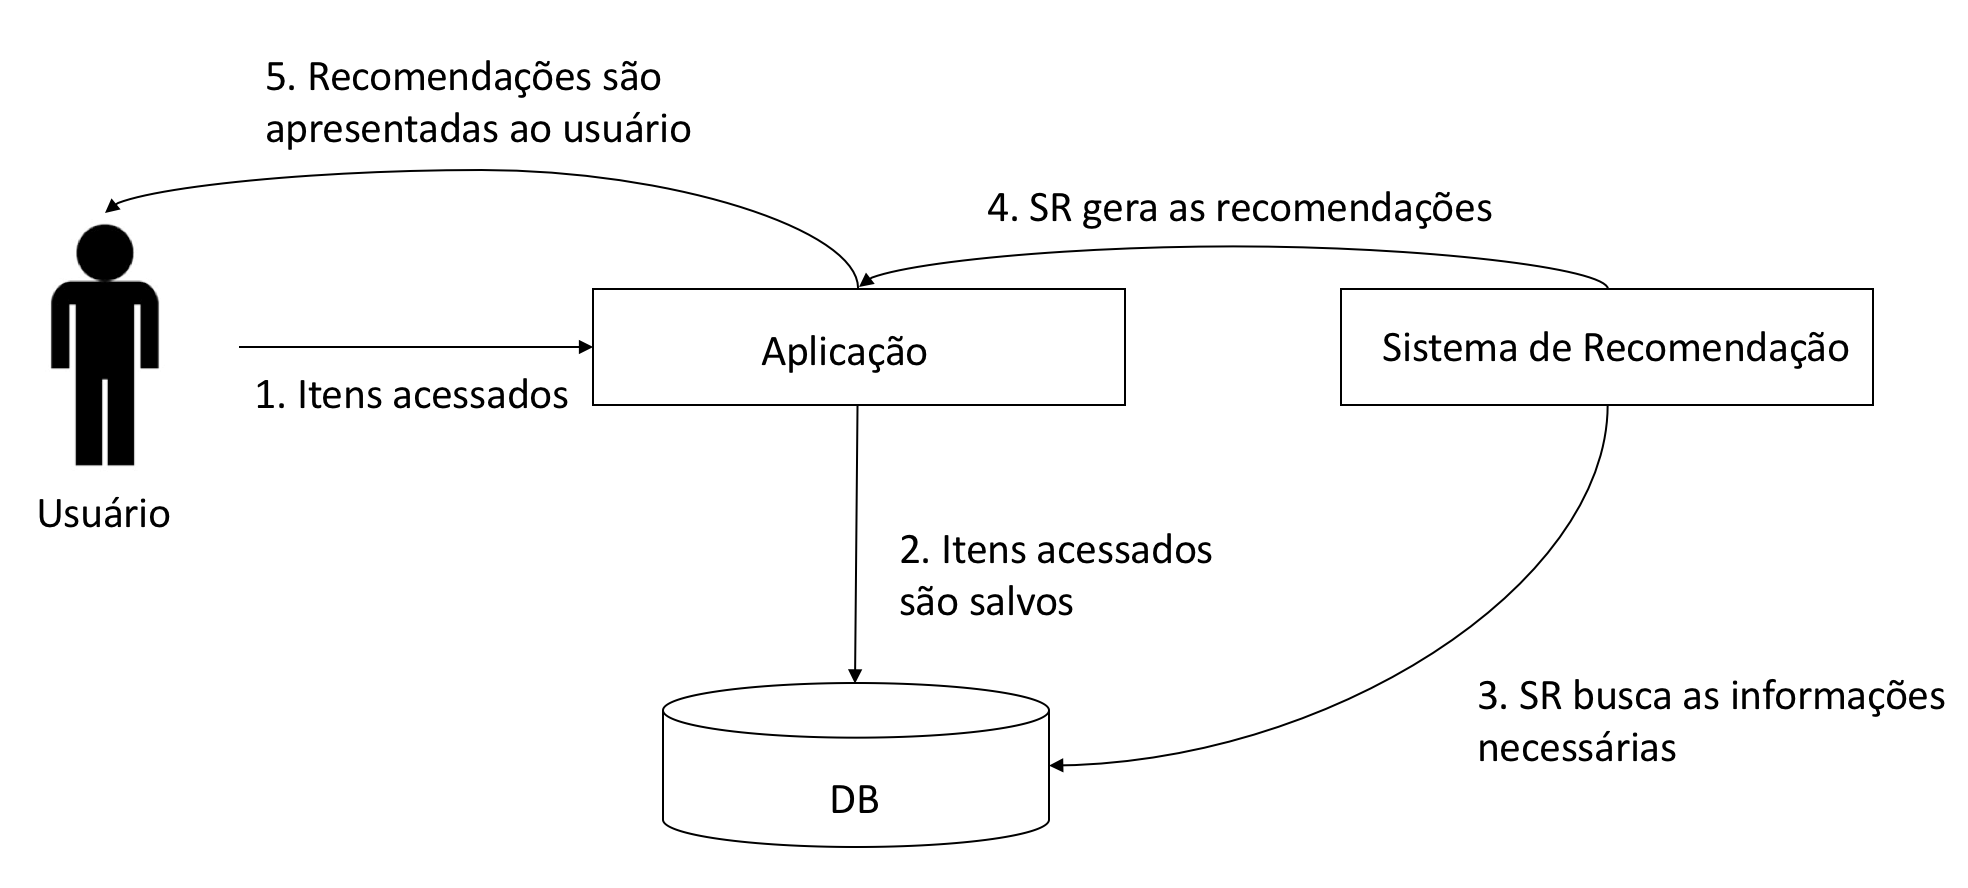
\includegraphics[scale=0.4]{./Figuras/modelo-proposta.png}
  \end{center}
  \legend{Fonte: O autor.}
\end{figure}

Na terceira etapa, o SR busca do Banco de Dados as informações necessárias para a recomendação, tanto sobre os itens
acessados pelo usuário quanto sobre os conjunto de itens que podem ser recomendados. Sobre os itens acessados, o SR
precisa das palavras-chave e a posição dos itens. Sobre os itens a serem recomendados, o SR precisa das palavras-chave
e se aqueles itens já foram acessados pelo usuário ou não. Após buscar essas informações, o SR aplica o algoritmo
mostrado anteriormente para gerar as recomendações, salva as recomendações geradas no Banco de Dados e retorna para a
Aplicação. A última etapa é responsabilidade da Aplicação, que prepara as recomendações para serem visualizadas pelo
usuário e as apresenta para ele.

\section{Cenário de Uso}

Um cenário de uso do Decaimento é apresentado a seguir. \textit{O aluno Pedro está matriculado em uma disciplina de Estrutura de Dados
que possui quatro tópicos, sendo eles Pilhas, Filas, Listas e Árvores. Nessa disciplina, para cada um dos conteúdos é
aplicada uma prova para avaliar os conhecimentos dos alunos. Para cada conteúdo da disciplina, existem 20 materiais que podem
ser acessados normalmente pelo aluno e mais 10 materiais relacionados que só podem ser acessados quando recomendados.
Cada um desses itens é representado pela palavra-chave do conceito em que está relacionado. Até o momento da primeira prova sobre o conteúdo de Pilhas,
Pedro acessou apenas materiais relacionados a Pilhas. O algoritmo de recomendação utilizando a abordagem Baseada em
Conteúdo recomenda para Pedro apenas materiais relacionados a Pilhas. Após a primeira prova, Pedro começa a acessar
materiais relacionados a Filas, o segundo tópico da disciplina. Em uma abordagem Baseada em Conteúdo tradicional as
recomendações continuariam sendo sobre o conteúdo de Pilhas por um bom tempo, pois o perfil de Pedro seria em grande
parte composto por materiais acessados sobre esse assunto. Porém, com o uso do \textbf{Decaimento}, no momento em que Pedro começar a
acessar materiais sobre Filas o algoritmo de recomendação dará um peso maior para esses materiais (sem ignorar os itens
acessados anteriormente) e em pouco tempo Pedro já estará recebendo recomendações sobre o novo tópico estudado. Da mesma
forma, se Pedro voltar a acessar conteúdos anteriores para relembrar algum conceito, o SR também perceberá isso e
recomendará itens relacionados ao primeiro conteúdo novamente.}

Agora é apresentado em mais detalhe o comportamento do algoritmo proposto no cenário de uso apresentado.
Ao estudar o primeiro assunto da disciplina, Pedro acessa conteúdos relacionados a Pilhas e no seu perfil
o SR formará o seu perfil com vários itens representados pela palavras-chave ``Pilha''. O SR, ao gerar uma recomendação,
irá encontrar um valor de similaridade alto entre o perfil do usuário e itens que também possuam
a palavra-chave ``Pilha''. Como todos os itens do perfil do usuário nesse momento tem a palavra-chave ``Pilha'', a recência não
terá um impacto importante nesse momento, pois todos os itens similares ao perfil do usuário terão a mesma recência. Na
Tabela \ref{tab:cenario-de-uso-1} é possível observar de forma resumida o comportamento do algoritmo (estamos considerando
que nenhum item candidato a recomendação tenha sido acessado).

\begin{table}[h]
\footnotesize
\caption[Cenário de Uso: comportamento do algoritmo após o acesso de itens relacionados a pilhas.]{Cenário de Uso: comportamento do algoritmo após o acesso de itens relacionados a pilhas.}
\label{tab:cenario-de-uso-1}
\centering
\begin{tabular}{|p{2cm}|p{2.5cm}|p{2.5cm}|p{2.5cm}|p{2.5cm}|}
  \hline
  \textbf{Funções} & \textbf{Item relacionado a pilhas} & \textbf{Item relacionado a filas} & \textbf{Item relacionado a listas} & \textbf{Item relacionado a árvores} \\
  \hline
  Similaridade & $1.0$ & $0.0$ & $0.0$ & $0.0$ \\
  \hline
  Recência & $1.0$ & $0.0$ & $0.0$ & $0.0$ \\
  \hline
  Acessado ou não & $1.0$ & $1.0$ & $1.0$ & $1.0$ \\
  \hline
  Relevância & $2.0$ & $1.0$ & $1.0$ & $1.0$ \\
  \hline
\end{tabular}
\legend{Fonte: O autor.}
\end{table}

Como é possível ver na Tabela \ref{tab:cenario-de-uso-1}, o item relacionado a pilhas terá uma maior
Relevância e será o item recomendado. A partir do momento que o usuário comece a acessar itens relacionados a filas,
o algoritmo passará a dar uma importância maior a itens relacionados a esse segundo tópico devido à recência desse tópico
para o perfil do usuário. Na Tabela \ref{tab:cenario-de-uso-2} é possível observar o comportamento do algoritmo nesse caso.

\begin{table}[h]
\footnotesize
\caption[Cenário de Uso: comportamento do algoritmo após o acesso de itens relacionados a filas.]{Cenário de Uso: comportamento do algoritmo após o acesso de itens relacionados a filas.}
\label{tab:cenario-de-uso-2}
\centering
\begin{tabular}{|p{2cm}|p{2.5cm}|p{2.5cm}|p{2.5cm}|p{2.5cm}|}
  \hline
  \textbf{Funções} & \textbf{Item relacionado a pilhas} & \textbf{Item relacionado a filas} & \textbf{Item relacionado a listas} & \textbf{Item relacionado a árvores} \\
  \hline
  Similaridade & $0.7$ & $0.3$ & $0.0$ & $0.0$ \\
  \hline
  Recência & $0.35$ & $1.0$ & $0.0$ & $0.0$ \\
  \hline
  Acessado ou não & $1.0$ & $1.0$ & $1.0$ & $1.0$ \\
  \hline
  Relevância & $1.245$ & $1.3$ & $1.0$ & $1.0$ \\
  \hline
\end{tabular}
\legend{Fonte: O autor.}
\end{table}

É possível observar na Tabela \ref{tab:cenario-de-uso-2} que, mesmo o perfil do usuário sendo ainda mais similar ao item
com a palavra-chave ``Pilha'', o impacto da Recência no algoritmo fez com a Relevância do item relacionado a filas
fosse maior e, dessa forma, esse item seja recomendado. Supondo que o aluno Pedro decida voltar a acessar itens
relacionados a pilhas, para recapitular os conteúdos, o comportamento do algoritmo nesse caso é apresentado na Tabela
\ref{tab:cenario-de-uso-3}.

\begin{table}[h]
\footnotesize
\caption[Cenário de Uso: comportamento do algoritmo após o aluno voltar a acessar itens relacionados a pilhas.]{Cenário de Uso: comportamento do algoritmo após o aluno voltar a acessar itens relacionados a pilhas.}
\label{tab:cenario-de-uso-3}
\centering
\begin{tabular}{|p{2cm}|p{2.5cm}|p{2.5cm}|p{2.5cm}|p{2.5cm}|}
  \hline
  \textbf{Funções} & \textbf{Item relacionado a pilhas} & \textbf{Item relacionado a filas} & \textbf{Item relacionado a listas} & \textbf{Item relacionado a árvores} \\
  \hline
  Similaridade & $0.75$ & $0.25$ & $0.0$ & $0.0$ \\
  \hline
  Recência & $1.0$ & $0.7$ & $0.0$ & $0.0$ \\
  \hline
  Acessado ou não & $1.0$ & $1.0$ & $1.0$ & $1.0$ \\
  \hline
  Relevância & $1.75$ & $1.175$ & $1.0$ & $1.0$ \\
  \hline
\end{tabular}
\legend{Fonte: O autor.}
\end{table}

Como pode ser observado na Tabela \ref{tab:cenario-de-uso-3}, algoritmo percebe que o aluno voltou a um tópico já
estudado anteriormente e voltaria a recomendar itens relacionados a isso. Como o perfil do aluno é composto ainda por
muitos itens relacionados ao tópico de Pilhas acessados primeiramente, ao voltar a acessar esses itens a relevância do item
relacionado a pilhas voltará a ser maior que o restante.

\section{Discussão Sobre o Algoritmo Proposto}

Um ponto negativo da Filtragem Colaborativa é a necessidade de uma comunidade de usuários ativa, que nem sempre é
possível em um AVA onde as turmas muitas vezes são menores (entre 10 e 100 alunos). A Abordagem Baseada
em Conteúdo é considerada para o SR proposto porque essa abordagem permite a recomendação em um sistema que não possui uma
comunidade ativa e pode suprir as necessidades desse domínio.

Os SRs Sensíveis ao Tempo têm uma vantagem em relação a outros SRs Sensíveis ao Contexto porque a informação temporal é
mais simples de capturar, manipular e processar que outras informações contextuais, e.g., localização. Além disso, esses tipos de
algoritmos estão sendo explorados em outros domínios de aplicação, como pode ser visto nos 88 artigos analisados no
Mapeamento Sistemático realizado \cite{de2017time}, e demonstraram bons resultados. Por isso, esse trabalho busca
aplicar o contexto temporal no algoritmo de recomendação na área educacional (na qual foram encontrados apenas quatro
trabalhos) e avaliar os resultados.

A escolha do Decaimento se justifica como forma de procurar minimizar uma das grandes desvantagens da abordagem Baseada em Conteúdo: a
Superespecialização. Na abordagem Baseada em Conteúdo as recomendações seriam geradas levando em conta todos os itens
acessados pelo usuário igualitariamente. Por outro lado, ao aplicar o Decaimento, os itens acessados mais recentemente possuem um
grau de importância maior para o algoritmo do que itens acessados anteriormente. Dessa forma, mesmo que o usuário
tenha acessado muitos materiais sobre determinado assunto, quando o usuário começar a acessar materiais sobre, outro assunto o algoritmo de
recomendação consegue rapidamente se adaptar e gerar recomendações sobre esse novo conteúdo.

O algoritmo proposto nesse trabalho considera o decaimento no peso dos itens do perfil do usuário em função da posição
do item na sequência de materiais acessados, como mostrado na Seção \ref{section:algoritmo-proposto}, e não na quantidade de tempo passada em
segundos como feito na maioria dos trabalhos relacionados mostrados no Capítulo \ref{chapter:trabalhos-relacionados}. Isso é uma vantagem, pois no domínio
educacional o passar do tempo não é tão relevante quanto em outros domínios, como na recomendação de \textit{Web Services} por
exemplo.

Os alunos em um AVA podem ter ritmos de estudo diferentes e, por isso, é assumido nesse trabalho que faz
mais sentido analisar quantos itens foram acessados desde do acesso de determinado material do que o tempo passado desde
a interação. Dessa forma, esse algoritmo não considera se o usuário acessou todos os itens do seu perfil em um
único dia, ou se ele acessou metade do materiais na primeira semana do curso e a outra metade na última semana ou se ele
acessou alguns materiais todos os dias durante o curso.

Além disso, no algoritmo proposto nesse trabalho não é definido um fator de decaimento único para os todos os usuários como nos trabalhos
relacionados apresentados no Capítulo \ref{chapter:trabalhos-relacionados}. Isto porque é necessário considerar
que cada aluno tem um estilo de aprendizagem diferente e o decaimento para um aluno poderia ser diferente do decaimento
para outros alunos. Vale ressaltar que não foram encontrados nos trabalhos relacionados que mostrem para calcular o fator
de decaimento de forma personalizada para cada usuário. Em geral, os autores utilizam o fator de decaimento escolhido de
forma empírica e aplicam o mesmo fator para todos os usuários.

O algoritmo proposto utiliza a abordagem Baseada em Conteúdo em
conjunto com o uso do tempo através da categoria Decaimento, ou seja, é dado um peso menor na recomendação para os
itens acessados há mais tempo pelo usuário e um peso maior para os itens mais recentes. No Sistema de Recomendação (SR)
proposto é combinada a similaridade entre o perfil do usuário e os itens, a recência dos itens acessados pelo usuário e
se os itens recomendados já foram ou não acessados. O Capítulo \ref{chapter:experimento} apresenta o experimento no qual
o algoritmo proposto foi avaliado.


